\section{D�coupage du projet}

\subsection{Vue d'ensemble du projet}
Le sch�ma suivant r�sume l'architecture applicative choisie � concevoir:

\begin{figure}
\centering
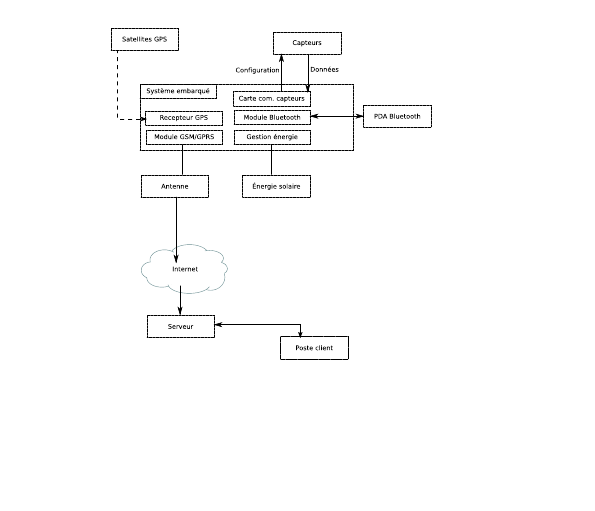
\includegraphics[width=8cm]{\PIXPATH/concep_generale}
\end{figure}
	
\subsection{D�coupage en sous-syst�mes}

Le syst�me peut alors �tre divis� en trois sous-syst�mes principaux :

\begin{enumerate}
\item Le syst�me embarqu�
\item Les serveurs (SSH, Sauvegarde, Web, ...)
\item Le service client (logiciel PDA/Smartphone) 
\end {enumerate}

Entre chaque sous-syst�me, nous avons une interface de communication, une API, 
qui se charge de les relier.

\begin{figure}
\centering
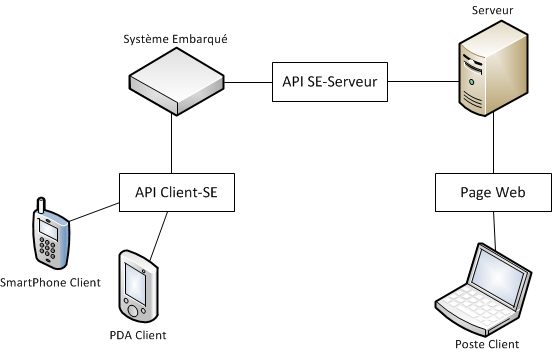
\includegraphics[width=8cm]{\PIXPATH/API}
\end{figure}

\subsection{Les sous-syst�mes}
Nous allons d�cliner la composition de chacun des sous-ensembles ci-dessus afin 
de donner une meilleure granularit� � la description.

\subsubsection{Syst�me Embarqu�}
\begin{enumerate}

\item Gestion des capteurs
Configuration/maintenance
Suivi des donn�es

\item Gestion de l'�nergie
Configuration/maintenance

\item Positionnement
Configuration/maintenance du module GPS
Suivi des donn�es (la position)

\item Communication avec les serveurs
Configuration/maintenance
Suivi des donn�es du syst�me embarqu�
Rapports de fonctionnement
Alertes

\item Communication Bluetooth
Configuration/maintenance
Suivi des donn�es des capteurs
Rapports de fonctionnement

\end{enumerate}


\subsubsection{Serveurs}
\begin{enumerate}
\item Serveur de Sauvegarde
Sauvegarde des enregistrements des capteurs dans la base de donn�es

\item Serveur HTTPS (Web)
Configuration des stations
Suivi donn�es provenant des stations

\item Serveur SSH (Communication avec le syst�me embarqu�)
Acquisition depuis les stations des enregistrements des capteurs
Configuration des stations
Maintenance logicielle � distance
Suivi des donn�es provenant des stations
\end{enumerate}


\subsubsection{Service client}
\begin{enumerate}
\item Application PDA/Smartphone
Configuration/maintenance
Suivi des donn�es
Rapports de fonctionnement

\item Application Web
Configuration/maintenance
Suivi des donn�es
Rapports de fonctionnement
\end{enumerate}
